\section{Introduction}
\subsection{Contexte de la problématique :}
Dans le cadre du projet de l'APP3 relatif au module réseaux de neurones nous allons nous intéresser aux réseaux de neurones récurrents. Nous allons prendre le rôle d'un stagiaire dans une entreprise oeuvrant dans le domaine de la réalité augmentée. Nous devrons utiliser des données d’accélération préalablement traitées provenant d’une centrale inertielle d’une montre intelligente et de les convertir en séquences de lettres. le but étant de faire une preuve de concept afin de déterminer si une technologie basée sur les réseaux de neurones récurrents est réalisable dans un contexte de ressources limitées.

\subsection{Description de la tâche à accomplir (traduction):}
\subsubsection{forme du Dataset :}
Notre sous-ensemble d'entrainement est organisé sous forme d'un dictionnaire. \\Chaque élément de ce dictionnaire est à son tour sous forme de liste contenant:
\begin{itemize}
    \item Une séquence cible (séquence de lettre : str = 'MOT')
    \item Une séquence d'entrée qui correspond aux coordonnées x et y de la centrale inertielle (un tableau de taille $\textsc{R}^{2*T}$).
\end{itemize}
Comme illustrer ci-dessous. 
$$
    Dataset = \Bigg\{\bigg[ \textsc{'mot'}, array \Big[(x_0,...,x_T), (y_0,...,y_T) \Big]\bigg],...\Bigg\}
$$
Lorsque l'on représente les données y en fonction de x nous avons alors la figure (\ref{fig:Figure 1  }) ci-dessous :
\begin{figure}[!h]
    \centering
    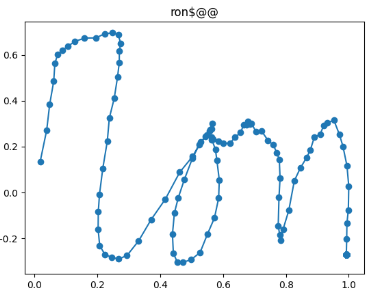
\includegraphics[width=60mm]{sections/inputSequence.PNG}
    \caption{Représentation des données de l'accéléromètre pour le mot : 'ron'}
    \label{fig:Figure 1  }
\end{figure}
\subsubsection{Tâche de traduction :}
Maintenant que nous connaissons la forme notre sous-ensemble nous devons trouver une façon d'associer nos séquences d'entrées aux séquences de sorties.\\
A priori, nous ne cherchons pas à génerer des nouvelles séquences de sorties à partir de notre séquence d'entrée (\textbf{Génération}), ni à associer la séquence d'entrée à une seul valeur cible (\textbf{Prédiction}), ni associer chaque élément de notre séquence d'entrée à une cible (\textbf{Annotation}). \\
En réalité, ce que nous cherchons à faire dans notre cas c'est d'associer une séquence d'entrée à sa séquence de sortie qui est de taille différente. Ceci correspond à la tâche de \textbf{Traduction}.
Nous devons donc traduire une séquence d'écriture cursive en texte.